\documentclass[a4paper]{article}
\usepackage{amsmath}
\usepackage{bm}
\usepackage{xcolor}
\usepackage{braket}
\usepackage{amssymb}
\usepackage{mathrsfs}
\usepackage{mathtools}
\begin{document}
	\title{Chapter\;13}
	\date{ }
	\maketitle
\section{generating function}
\subsection{n point Green function}
Define n point Green function $\tilde{G}^{(n)}(k_1,\cdots,k_n)$
$$\tilde{G}^{(n)}(k_1,\cdots,k_n)=\text{sum of all diagrams with n external meson lines}$$Meson lines mean that these external lines are gengerated by mesons.For example,diagram for a four point Green function can be drawn like
\begin{figure}[htbp]
	\centering
	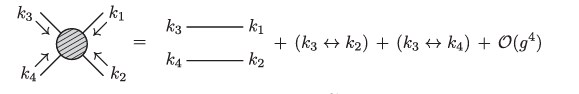
\includegraphics[width=0.6\textwidth]{19.png}
	\caption{four point Green function}
\end{figure}

then
\begin{align*}
	\tilde{G}^{(4)}(k_1,k_2,k_3,k_4)&=(2\pi)^4\delta^{(4)}(k1_+k_3)\frac{i}{k_1^2-m^2+i\epsilon}\\&\times(2\pi)^4\delta^{(4)}(k_2+k_4)\frac{i}{k_4^2-m^2+i\epsilon}\\&+\text{permutation terms}+\text{higher order terms}
\end{align*}
Generally,for an n point Green function,conventions are summarized to be
\begin{figure}[htbp]
	\centering
	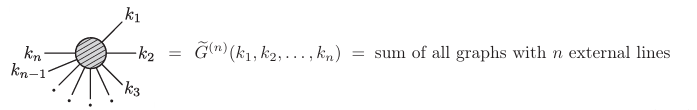
\includegraphics[width=0.6\textwidth]{20.png}
	\caption{n point Green function}
\end{figure}

\par (1)The momenta $k_i$ are oriented inward.
\par (2)The external lines include propagators $\frac{i}{k_i^2-m^2+i\epsilon}$.
\par (3)All four-momentum conserving delta functions are included.
\par (4)All connected and disconnected are included.
\vspace{0.02\textheight}
\par One can also define $G^{(n)}(x_1,\cdots,x_n)$ as inverse Fourier transform of $\tilde{G}^{(n)}(k_1\cdots,k_n)$ 
$$G^{(n)}(x_1,\cdots,x_n)=\int\frac{d^4k_1}{(2\pi)^4}\cdots\frac{d^4k_1}{(2\pi)^4}e^{-ik_1\cdot x_1-\cdots-ik_n\cdot x_n}\tilde{G}^{(n)}(k_1\cdots,k_n)$$.
\subsection{generating functional for $G^{(n)}(x_i)$}
Given the Hamiltonian density $\mathscr{H}$ of the system,define a new Hamiltonian density $\mathscr{H}'$ by adding a source term to the old one.$$\mathscr{H}'=\mathscr{H}+\rho(x)\phi(x)$$Now all the so called external lines are defined to be those meson lines caused by source term while meson lines in the old Hamiltonian density are excluded.For an external line with label momenta $k$,it looks like
\begin{figure}[htbp]
	\centering
	
\includegraphics[width=0.6\textwidth]{21.png}
	\caption{external line for $\rho(x)\phi(x)$}
\end{figure}

where $\tilde{\rho}(k)$ is Fourier transform of $\rho(x)$.$k$ in oriented inward(inside structure is not demonstrated) sourcing from black dot.
\par Now define generating funcctional $\mathscr{Z}[\rho]$ for n point Green function.
$$\mathscr{Z}[\rho]\equiv1+\sum_{n=1}^{\infty}\frac{(-i)^n}{n!}\int\frac{d^4k_1}{(2\pi)^4}\cdots\frac{d^4k_1}{(2\pi)^4}\tilde{G}^{(n)}(k_1,\cdots,k_n)\tilde{\rho}(-k_1)\cdots\tilde{\rho}(-k_n)$$
Also,it is also the definition of matrix element $\bra{0}S\ket{0}$ in the presence of $\rho$,which is denoted as $\bra{0}S\ket{0}_{\rho}$.
\par By Parseval's Theorem,the generating function can be expressed in terms of space-time variables$$\mathscr{Z}[\rho]\equiv1+\sum_{n=1}^{\infty}\frac{(-i)^n}{n!}\int d^4x_1\cdots d^4x_nG^{(n)}(x_1,\cdots,x_n)\rho(x_1)\cdots\rho(x_n)$$
Then n point Green function can be found by taking variation of generating function
$$G^{(n)}(x_1,\cdots,x_n)=i^n\frac{\delta^n\mathscr{Z}[\rho]}{\delta\rho(x_1)\cdots\delta\rho(x_n)}\Big|_{\rho(x)=0}$$
Also define connected generating functiong that only takes care about connected diagrams
$$\mathscr{Z}_C[\rho]\equiv1+\sum_{n=1}^{\infty}\frac{(-i)^n}{n!}\int d^4x_1\cdots d^4x_nG^{(n)}_C(x_1,\cdots,x_n)\rho(x_1)\cdots\rho(x_n)$$
which is equal to $ln\mathscr{Z}[\rho]$.(Recall that sum of all = $e^{\text{sum of connected}}$)Sometimes,the notation $W[\rho]=\frac{\mathscr{Z}_C[\rho]}{i}$ is also used.
\section{scattering without adiabatic function }
with the method of generating function,turn-on-and-off function can retreat from calculation of scattering amplitude.Let  $\ket{\Omega}$ denote $\ket{0}^P$,the physical vacuum.Now redefine generating function$$\mathscr{Z}[\rho]=\bra{\Omega}U_{I}(\infty,-\infty)\ket{\Omega}$$which is different from the previous one,just abuse of notation.The physical vacuum satisfies
\begin{align*}
	&H\ket{\Omega}=0\\
	&\braket{\Omega|\Omega}=1
\end{align*}
Now source term is treated as interaction part,thus $"\phi_I(x)=\phi_H(x)"$,the interaction picture in presence of source term is equal to the Heisenberg picture in absence of source term.Thus$$U_I(\infty,-\infty)=Te^{-i\int d^4x\rho(x)\phi_H(x)}$$Substitute this into  expression of generating function$$\mathscr{Z}[\rho]=\sum_{n=0}^{\infty}\frac{(-i)^n}{n!}\int d^4x_1\cdots d^4x_n\rho(x_1)\cdots\rho(x_n)\bra{\Omega}T[\phi_H(x_1)\cdots\phi_H(x_n)]\ket{\Omega}$$Therefore,n point Green function generated from this $\mathscr{Z}[\rho]$ is$$G^{(n)}(x_1,\cdots,x_n)=\bra{\Omega}T[\phi_H(x_1)\cdots\phi_H(x_n)]\ket{\Omega}$$
Now consider another generating function $\mathscr{Z}[\rho]^{Feyn}$,which is computed by summing all the diagrams with external legs(of course contributed by source term).The proper expression for this generating function is$$\mathscr{Z}[\rho]^{Feyn}=\lim_{\substack{t_+\rightarrow+\infty \\ t_-\rightarrow-\infty}}\frac{\bra{0}Te^{-i\int_{t_-}^{t_+}d^4x(\mathscr{H}_I+\rho\phi_I)}\ket{0}}{\bra{0}Te^{-i\int_{t_-}^{t_+}d^4x\mathscr{H}_I}\ket{0}}$$
The subscript $I$ here refers to interaction picture in the absence of source term.This expression makes sense,as the denominator actually cancels out all the solely separated diagrams contributed by $\mathscr{H}$.Only thing that is left is those diagrams whose outside is external lines contributed by source terms and inside is regular Feynman diagram contributed by $\mathscr{H}$.
\par Taylor expand the expression and find that the Green function generated by it is$$G^{(n)Feyn}(x_1,\cdots,x_n)=\lim_{\substack{t_+\rightarrow+\infty \\ t_-\rightarrow-\infty}}\frac{\bra{0}Te^{-i\int_{t_-}^{t_+}d^4x\mathscr{H}_I}\phi_I(x_1)\cdots\phi_I(x_n)\ket{0}}{\bra{0}Te^{-i\int_{t_-}^{t_+}d^4x\mathscr{H}_I}\ket{0}}$$With a bit of mathematical efforts,it can be shown that$$\mathscr{Z}[\rho]=\mathscr{Z}[\rho]^{Feyn} \text{ and } G^{(n)}(x_1\cdots,x_n)=G^{(n)Feyn}(x_1\cdots,x_n)$$
\section{construct in and out state}
There is one problem remained,construction of in and out state.Previously with adiabatic function,one can construct in and out state based on that real state asmyptotically behaves like free state in the distant past and future.But when adiabatic function is abolished,this conception is not valid.
\subsection{renormalized field}
For the sake of better discussion,introduce a new field dependent of 4-momentum $k$ and only $k^2$ based on the old one
$$\phi'(x)\equiv\frac{\phi_H(x)-\bra{\Omega}\phi_H(x)\ket{\Omega}}{\sqrt{Z_3}}$$where $Z_3$ satisfies $\bra{\Omega}\phi_H(x)-\bra{\Omega}\phi_H(x)\ket{\Omega}\ket{\Omega}=\sqrt{Z_3}$ so that$$\bra{k}\phi'(x)\ket{\Omega}=e^{ik\cdot x}$$for any single particle state $\ket{k}$.And $\phi'(x)$ is called renormalized field.
\subsection{creation operator}
Define normalized wave packet states:$$\ket{f}\equiv\int\frac{d^3\bm{k}}{(2\pi)^32\omega_{\bm{k}}}F(\bm{k})\ket{k}$$with dispersion relationship $k^2=\mu^2$.
Associated with each of these states is a function $f(x)$,$$f(x)\equiv\int\frac{d^3\bm{k}}{(2\pi)^32\omega_{\bm{k}}}F(\bm{k})e^{-ik\cdot x}$$which satisfies k-G equation:$(\Box^2+\mu^2)f(x)=0$.
\par Now also define a quantity depending on and only on $f(x)$ and time $t$
$$\phi'^{f}(t)\equiv i\int d^3\bm{x}[\phi'(x)\partial_0f(x)-f(x)\partial_0\phi'(x)]$$
Now claim two things that can prove without much efforts:
\begin{align*}
	&\braket{k|f}=F(\bm{k})\\
	&\bra{k}\phi'^f(t)\ket{\Omega}=F(\bm{k})
\end{align*}
for any 4-momenum $k$.Thus$$\phi'^f(t)\ket{\Omega}=\ket{f}$$ $\phi'^f(t)$ acts like a creation operator for normalized state $\ket{f}$.
\par Futhermore,one can prove that for any state $\ket{\psi}$:$$\lim_{t\rightarrow\pm\infty}\bra{\psi}\phi'^f(t)\ket{\Omega}=\braket{\psi|f}$$Therefore,$\phi'^f(t)$ indeed is the creation operator that creates normalized state $\ket{f}$ in distant past or future.One can create any kind of such state as long as choosing $f(x)$ properly. 
\end{document}